\documentclass[runningheads]{llncs}\usepackage{knitr}
\usepackage{graphicx}
\usepackage[utf8]{inputenc}
\usepackage[spanish]{babel}
\usepackage{xspace}
\newcommand{\mytilde}{\lower.80ex\hbox{\char`\~}\xspace}
\IfFileExists{upquote.sty}{\usepackage{upquote}}{}
\begin{document}

\title{metR - Visualización y manejo de campos meteorológicos}

%\titlerunning{Abbreviated paper title}
% If the paper title is too long for the running head, you can set
% an abbreviated paper title here
%
\author{Elio Campitelli}

%
\authorrunning{E. Campitelli}
% First names are abbreviated in the running head.
% If there are more than two authors, 'et al.' is used.
%
\institute{Centro de Investigaciones del Mar y la Atmósfera - CONICET\\
\email{elio.campitelli@cima.fcen.uba.ar}\\
%\url{http://www.springer.com/gp/computer-science/lncs}
}
%
\maketitle              % typeset the header of the contributions
%
% \begin{abstract}
\keywords{meteorología \and tidy data \and visualización de datos}
% \end{abstract}




Gran parte de la investigación en ciencias de la atmósfera consiste en el análisis y visualización de datos. Uno de los softwares de visualización de datos más utilizado por la comunidad meteorológica y oceanográfica es GrADs (Grid Analysis and Display System), el cual permite leer y graficar campos escalares y vectoriales con gran facilidad. Sin embargo, su lenguaje de scripting es muy limitado, carece de capacidades estadísticas nativas y no existen gran cantidad de extensiones que las implementen. R, en cambio, posee implementaciones de virtualmente cualquier tratamiento estadístico usado en ciencias de la atmósfera. Sin embargo, con el paquete \texttt{raster} --el más usado para leer y graficar datos geográficos-- los datos quedan relativamente ocultos detrás de una estructura opaca que no facilita la interacción con otros paquetes; en particular, no es posible graficarlos utilizando \texttt{ggplot2}. 

La finalidad de \texttt{metR} es proveer facilidades en la lectura, manejo y visualización de datos meteorológicos en R utilizando estructuras comunes soportadas por la mayoría de los paquetes, de manera de poder beneficiarse de los aportes de la comunidad. Hace fuerte uso de \texttt{data.table} por su eficiencia en uso de memoria y velocidad (importante dada la gran cantidad de datos que suelen usarse en meteorología), y en \texttt{ggplot2} por su flexibilidad y facilidad en la creación de gráficos. 

En su extensión de \texttt{ggplot2}, \texttt{metR} provee \texttt{geoms} para graficar contornos llenos, contornos de Tanaka, líneas de corriente, vectores y mapas de relieve, y escalas específicas que facilitan la creación de mapas y cortes verticales. En lo que refiere a manejo de datos, provee funciones para lectura datos desde archivos NetCDF directamente en \texttt{data.frames}, cálculo de valores principales, imputación de datos faltantes, transformada de Fourier y derivadas. Además, tiene funciones específicas de física atmosférica, como la ley de gases ideales, relaciones de procesos adiabáticos, presión de saturación del vapor de agua, fuerza de coriolis y otros.

\texttt{metR} está en estado experimental y de activo desarrollo, tanto en crecimiento de funcionalidad como en refinamiento de interfaces y corrección de errores. Como todo proyecto de código abierto, es deseable además que a medida que sea adoptado por la comunidad, surgan nuevos casos de uso que incentiven su evolución más allá de las necesidades personales de un sólo desarrollador.

\textbf{Ejemplo}. Se calculan las anomalías temporales para cada puntos de grilla y calcular el campo asociado a la primera componente principal para cada mes. Finalmente, se calcula el viento geostrófico correspondiente a ese campo. Todo este proceso toma unas pocas líneas de código y se integra sin esfuerzo en el \emph{workflow} de \texttt{data.table}. 

\begin{knitrout}
\definecolor{shadecolor}{rgb}{0.969, 0.969, 0.969}\color{fgcolor}\begin{kframe}
\begin{alltt}
\hlstd{geopotential[, gh.t} \hlkwb{:=} \hlkwd{Anomaly}\hlstd{(gh),} \hlkwc{by} \hlstd{=} \hlkwd{.}\hlstd{(lon, lat,} \hlkwd{month}\hlstd{(date))]}
\hlstd{geopotential[, gh.t.w} \hlkwb{:=} \hlstd{gh.t}\hlopt{*}\hlkwd{sqrt}\hlstd{(}\hlkwd{cos}\hlstd{(lat}\hlopt{*}\hlstd{pi}\hlopt{/}\hlnum{180}\hlstd{))]}
\hlstd{eof} \hlkwb{<-} \hlstd{geopotential[,} \hlkwd{EOF}\hlstd{(gh.t.w} \hlopt{\mytilde} \hlstd{date} \hlopt{|} \hlstd{lon} \hlopt{+} \hlstd{lat,} \hlkwc{n} \hlstd{=} \hlnum{1}\hlstd{)}\hlopt{$}\hlstd{right,}
                    \hlkwc{by} \hlstd{=} \hlkwd{month}\hlstd{(date)]}
\hlstd{eof[,} \hlkwd{c}\hlstd{(}\hlstr{"u"}\hlstd{,} \hlstr{"v"}\hlstd{)} \hlkwb{:=} \hlkwd{GeostrophicWind}\hlstd{(gh.t.w, lon, lat),} \hlkwc{by} \hlstd{= month]}
\end{alltt}
\end{kframe}
\end{knitrout}

Luego, se grafica el campo de geopotencial con contornos llenos de manera que haya una relación uno a uno entre los niveles graficados y los señalados en la escala de colores. El campo de movimiento, por su parte, se grafica con líneas de corriente. 

\begin{knitrout}
\definecolor{shadecolor}{rgb}{0.969, 0.969, 0.969}\color{fgcolor}\begin{kframe}
\begin{alltt}
\hlstd{binwidth} \hlkwb{<-} \hlnum{0.01}
\hlkwd{ggplot}\hlstd{(eof[month} \hlopt \hlnum{1}\hlstd{],} \hlkwd{aes}\hlstd{(lon, lat))} \hlopt{+}
   \hlkwd{geom_contour_fill}\hlstd{(}\hlkwd{aes}\hlstd{(}\hlkwc{z} \hlstd{= gh.t.w),} \hlkwc{circular} \hlstd{=} \hlstr{"x"}\hlstd{,}
                     \hlkwc{breaks} \hlstd{=} \hlkwd{AnchorBreaks}\hlstd{(}\hlnum{0}\hlstd{, binwidth,} \hlnum{0}\hlstd{))} \hlopt{+}
   \hlkwd{geom_streamline}\hlstd{(}\hlkwd{aes}\hlstd{(}\hlkwc{dx} \hlstd{=} \hlkwd{dlon}\hlstd{(u, lat),} \hlkwc{dy} \hlstd{=} \hlkwd{dlat}\hlstd{(v)),} \hlkwc{L} \hlstd{=} \hlnum{30}\hlstd{,}
                   \hlkwc{skip} \hlstd{=} \hlnum{2}\hlstd{,} \hlkwc{circular} \hlstd{=} \hlstr{"x"}\hlstd{)} \hlopt{+}
   \hlkwd{scale_fill_divergent}\hlstd{(}\hlkwc{breaks} \hlstd{=} \hlkwd{AnchorBreaks}\hlstd{(}\hlnum{0}\hlstd{, binwidth,} \hlnum{0}\hlstd{),}
                        \hlkwc{guide} \hlstd{=} \hlstr{"colorstrip"}\hlstd{,} \hlkwc{name} \hlstd{=} \hlstr{""}\hlstd{)} \hlopt{+}
   \hlkwd{scale_y_latitude}\hlstd{(}\hlkwc{ticks} \hlstd{=} \hlnum{15}\hlstd{)} \hlopt{+} \hlkwd{scale_x_longitude}\hlstd{()} \hlopt{+} \hlstd{geom_map} \hlopt{+}
   \hlkwd{coord_quickmap}\hlstd{(}\hlkwc{xlim} \hlstd{=} \hlkwd{c}\hlstd{(}\hlnum{0}\hlstd{,} \hlnum{360}\hlstd{),} \hlkwc{ylim} \hlstd{=} \hlkwd{c}\hlstd{(}\hlopt{-}\hlnum{90}\hlstd{,} \hlopt{-}\hlnum{20}\hlstd{))} \hlopt{+}
   \hlkwd{theme_minimal}\hlstd{()} \hlopt{+} \hlkwd{theme_field}\hlstd{()}
\end{alltt}
\end{kframe}\begin{figure}
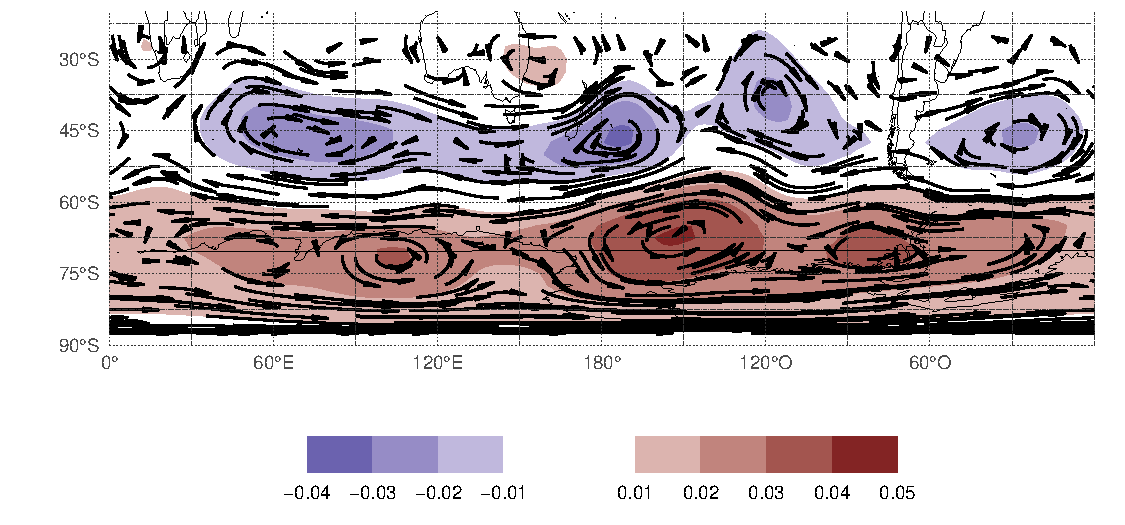
\includegraphics[width=\maxwidth]{figure/example-plot-1} \caption[Anomalía de altura geopotencial media en contornos llenos (mgp) y viento geostrófico en líneas de corriente]{Anomalía de altura geopotencial media en contornos llenos (mgp) y viento geostrófico en líneas de corriente.}\label{fig:example-plot}
\end{figure}


\end{knitrout}


% \section{Limitaciones}
% 
% El uso de `data.table`s para el manejo de datos implica una importante limitación para \texttt{metR}. Muchas aplicaciones meteorológicas hacen uso de cantidades de datos que resultan imposibles cargar en memoria RAM en la mayoría de las computadoras personales. \texttt{metR} tampoco puede manejar campos que no se encuentren en en grillas regulares o en grillas proyectadas. En ambos casos paquetes como \texttt{raster} y \texttt{rasterVis} son indispensables. 
% 



\end{document}
